\documentclass{article}
\usepackage{ctex}
\usepackage[utf8]{inputenc}
\title{Engineering Optimization Homework}
\author{Tai Jiang}
\date{March 2024}
\usepackage{amsmath}
\usepackage{amsthm}
\usepackage{amssymb}
\usepackage{tikz}
\usepackage{graphicx}
\usetikzlibrary{automata, positioning}
\usepackage{color}
\usepackage{listings}


\begin{document}
  \maketitle
  \section{Nature of OR}
  Maximize $Z = 2x_1 + 5x_2$

  
  subject to
  \begin{itemize}
    \item $10x_1 + 30x_2 \leq 30$
    \item $95x_1 - 30x_2 \leq 75$
  \end{itemize}

  and

  $x_1$, $x_2$ are binary
  
  \paragraph{Answer}:

  \paragraph{$x_1=0$}:

  Maximize $Z = 5x_2$

  subject to

  \begin{equation*}
    \begin{aligned}
      x_2 \leq 1 \\
      30x_2 \geq -75
    \end{aligned}
  \end{equation*}


  $(x_1, x_2) = (0, 1)$ with $Z=5$

  \paragraph{$x_1=1$}:

  Maximize $Z = 2 + 5x_2$

  subject to

  \begin{equation*}
    \begin{aligned}
      30x_2 \leq 20 \\
      30x_2 \geq 20
    \end{aligned}
  \end{equation*}

  $(x_1, x_2) = (1, \frac{2}{3})$ with $Z=5 \frac{1}{3}$

  \paragraph{$x_2=0$}:

  Maximize $Z = 2x_1$

  
  subject to

  \begin{equation*}
    \begin{aligned}
      x_1  \leq 3 \\
      95x_1 \leq 75
    \end{aligned}
  \end{equation*}

  $(x_1, x_2) = (\frac{15}{19}, 0)$ with $Z=1 \frac{11}{19}$

  \paragraph{$x_2=1$}:

  Maximize $Z = 2x_1 + 1$

  
  subject to

  \begin{equation*}
    \begin{aligned}
      x_1  \leq 0 \\
      95x_1 \leq 105
    \end{aligned}
  \end{equation*}

  $(x_1, x_2) = (0, 1)$ with $Z=1$



  \begin{figure}[ht]
    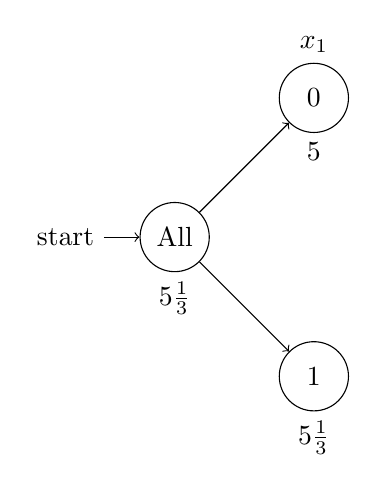
\begin{tikzpicture}[node distance=2.5cm, on grid]
      \node[state, initial] (q0) {All};
      \node[below] at (q0.south) {$5\frac{1}{3}$};
      \node[state, above right=of q0] (q10) {0};
      \node[above] at (q10.north) {$x_1$};
      \node[below] at (q10.south) {5};
      \node[state, below right=of q0] (q11) {1};
      \node[below] at (q11.south) {$5\frac{1}{3}$};
      \path[->]
        (q0) edge node {} (q10)
        (q0) edge node {} (q11);
    \end{tikzpicture}
  \end{figure}

  \begin{figure}[ht]
    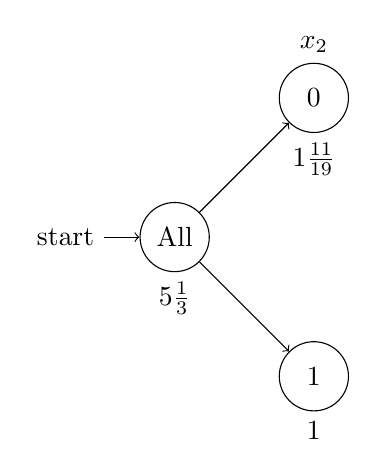
\begin{tikzpicture}[node distance=2.5cm, on grid]
      \node[state, initial] (q0) {All};
      \node[below] at (q0.south) {$5\frac{1}{3}$};
      \node[state, above right=of q0] (q20) {0};
      \node[above] at (q20.north) {$x_2$};
      \node[below] at (q20.south) {$1\frac{11}{19}$};
      \node[state, below right=of q0] (q21) {1};
      \node[below] at (q21.south) {1};
    
      \path[->]
        (q0) edge node {} (q20)
        (q0) edge node {} (q21);
    \end{tikzpicture}
  \end{figure}

\end{document}